% !TeX root = chapter-6-7-8.tex

\selectlanguage{hebrew}

\begin{comment}

\chapter{חשבון דיפרנציאלי ואינטגרלי}

\end{comment}

%%%%%%%%%%%%%%%%%%%%%%%%%%%%%%%%%%%%%%%%%%%%%%%%%%%%%%%%%%%%%%%%%%%%%%

\section{קיץ תשע"ז מועד ב}

\begin{center}
\selectlanguage{english}
\includegraphics[width=\textwidth]{summer-2017b-7a}
\includegraphics[width=\textwidth]{summer-2017b-7b}
\end{center}

\vspace{-2ex}

\textbf{סעיף א}

הגרף
$I$
מתאפס בנקודה 
$C$
שם לגרף 
$II$
יש נקודה מקסימלית, ומתאפס בציר ה-%
$y$
שם לגרף יש נקודה מינימלית. לכן,
$II$
הוא הגרף של
$f(x)$
ו-%
$I$
הוא הגרף של
$f'(x)$.

\textbf{סעיף ב}

בנקודת פיתול הנגזרת השנייה מתאפסת:
\erh{2pt}
\begin{equationarray*}{rcl}
f''(x) &=& x\cdot 3(x+b)^2+1\cdot (x+b)^2=(x+b)^2(4x+b)\\
f''(-1) &=& (b-1)^2 (b-4)=0\\
b&=&4\,,
\end{equationarray*}
כי נתון ש-%
$b>1$.

\np

\textbf{סעיף ג}

הערך המקסימלי יתקבל כאשר הנגזרת של ההפרש מאפסת:
\erh{2pt}
\begin{equationarray*}{rcl}
(f(x)-f'(x))'&=& f'(x) - (x(x+4))^3)'\\
&=&x(x+4)^3 - x\cdot 3(x+4)^2 - 1\cdot (x+4)^3\\
&=&(x+4)^2(x^2-4)=0\,.
\end{equationarray*}
הפתרונות הם
$x=-4,x=\pm 2$.
הערך היחיד בתחום בין
$x_C=-4$
ל-%
$x_D=1-\sqrt{5}$
הוא
$-2$. 
נבדוק:
$-2<1-\sqrt{5}=-1.24$.

\begin{comment}

\np

%%%%%%%%%%%%%%%%%%%%%%%%%%%%%%%%%%%%%%%%%%%%%%%%%%%%%%%%%%%%%%%%%%%%%%

\section{קיץ תשע"ז מועד א}

\begin{center}
\selectlanguage{english}
\includegraphics[width=\textwidth]{summer-2017a-7}
\end{center}

\vspace{-2ex}

\textbf{סעיף א}

$(1)$
הפונקציה מוגדרת כאשר המכנה לא מתאפס, כאשר 
$x \neq \frac{\pi}{2} \pm n\pi$.

$(2)$
נקודות החיתוך עם ציר ה-%
$x$
הן כל הנקודות עבורן
$\sin x = 0, \cos x \neq 0$,
שהן 
$x=\pm n\pi$.
כאשר 
$x=0$,
$y=0$
והנקודה היא גם נקודת חיתוך עם ציר ה-%
$x$.

$(3)$
כאשר
$x=\frac{\pi}{2} \pm n\pi$,
הפונקציה לא מוגדרת כי ערכה אינסופי, ולכן הן 
\asms{}
אנכיות. אין 
\asm{}
אופקיות כי ערך הפונקציה לא חסום כאשר 
$x\longrightarrow\pm\infty$.


$(4)$
\[
f'(x)=\frac{2\cos x\cdot\cos^3 x - 2\sin x \cdot 3\cos^2 x \cdot -\sin x}{\cos^6 x}=\frac{2\cos^2 x + 6\sin^2 x}{\cos^4 x}\,,
\]
כאשר צימצמנו 
$\cos^2 x$
בתחום ההגדרה. כל הגורמים בביטוי חיוביים ולכן הפונקציה עולה בכל תחום ההגדרה.

\np

\textbf{סעיף ב}

\begin{center}
\selectlanguage{english}
\begin{tikzpicture}%[scale=.8]
\begin{axis}[
    trig format plots=rad,
    axis lines=center,
    xmin = -2,
    xmax = 5,
    xtick={-1.57,0,1.57,3.14,4.71},
    xticklabels={$-\frac{\pi}{2}$,$0$, $\frac{\pi}{2}$,$\pi$,$\frac{3\pi}{2}$},
    ymin = -10,
    ymax = 10,
    ymajorticks=false,
    xticklabel style={anchor=north west,},
]
\addplot [
    domain=-1.4:1.4,
    samples=50, 
]
{(2*sin(x))/(cos(x)^3)};
\addplot [
    domain=1.7:4.55,
    samples=50, 
]
{(2*sin(x))/(cos(x)^3)};
\draw[dashed,thick] (axis cs:-1.57,-10) -- (axis cs:-1.57,10);
\draw[dashed,thick] (axis cs:1.57,-10) -- (axis cs:1.57,10);
\draw[dashed,thick] (axis cs:4.71,-10) -- (axis cs:4.71,10);
\fill (axis cs:0,0) circle(1.5pt);
\fill (axis cs:3.14,0) circle(1.5pt);
\end{axis}
\end{tikzpicture}
\end{center}


\textbf{סעיף ג}
\[
\int_0^a \frac{2\sin x}{\cos^3 x}dx = \left. \cos^{-2} x \right|_0^a=\frac{1}{\cos^2 a}-\frac{1}{1^2}=1\,.
\]
מכאן ש-%
$\cos a=\sqrt{\frac{1}{2}}=\frac{\sqrt{2}}{2}$,
והפתרון היחיד בתחום
$0<a<\frac{\pi}{2}$
הוא
$a=\frac{\pi}{4}$.
\np

%%%%%%%%%%%%%%%%%%%%%%%%%%%%%%%%%%%%%%%%%%%%%%%%%%%%%%%%%%%%%%%%%%%%%%

\section{קיץ תשע"ה מועד ב}

\begin{center}
\selectlanguage{english}
\includegraphics[width=\textwidth]{summer-2015b-7}
\end{center}

\vspace{-2ex}

\textbf{סעיף א}

\[
f(x)=\int f'(x) dx = \int \frac{1}{2}(x^2+9)^{-\frac{1}{2}}\cdot 2x\: dx = (x^2+9)^{\frac{1}{2}} +c\,.
\]
לפי הנתון,
$\sqrt{0^2+9}+c=3$,
ולכן
$c=0$
ו-%
$f(x) = \sqrt{x^2+9}$.

\textbf{סעיף ב}

$(1)$
$f(x)$
מוגדרת עבור כל
$x$
כי הערך של
$x^2+9$
חיובי. מאותה סיבה, המכנה של
$f'(x)$
תמיד חיובי ו-%
$f'(x)$
מוגדרת עבור כל 
$x$.


$(2)$
$f'(x)$
מוגדרת עבור כל 
$x$
אז אין
\asms{}
אנכיות. ה%
\asms{}
האופקיות הן:
\[
\frac{\disfrac{x}{x}}{\sqrt{1+\disfrac{9}{x^2}}}\limit{+\infty}+1,\quad\quad
\frac{\disfrac{x}{x}}{-\sqrt{1+\disfrac{9}{x^2}}}\limit{-\infty}-1\,.
\]

\np

$(3)$
על ידי הצבה של
$x=0$
יש נקודת חיתוך ב-%
$(0,0)$.
המכה חיובי לכן 
$y=0$
רק אם 
$x=0$
וכבר קיבלנו נקודת חיתוך זו.

$(4)$
\[
f''(x)= \frac{1\cdot\sqrt{x^2+9}- x\cdot \disfrac{1}{2} \disfrac{1}{\sqrt{x^2+9}}\cdot 2x}{x^2+9}=\frac{9}{(x^2+9)\sqrt{x^2+9}}\,.
\]
הנגזרת השנייה תמיד חיובי ולכן הנגזרת הראשונה עולה בכל התחום.

$(5,6)$

\begin{center}
\selectlanguage{english}
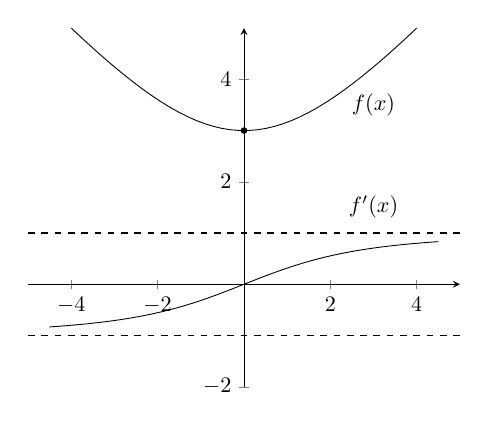
\begin{tikzpicture}[scale=.8]
\begin{axis}[
    axis lines=center,
    xmin = -5,
    xmax = 5,
    ymin = -2,
    ymax = 5,
]
\addplot [
    domain=-5:5,
    samples=50, 
]
{sqrt(x^2+9)};
\addplot [
    domain=-4.5:4.5,
    samples=50, 
]
{(x)/(sqrt(x^2+9))};
\draw[dashed,thick] (axis cs:-5,1) -- (axis cs:5,1);
\draw[dashed,thick] (axis cs:-5,-1) -- (axis cs:5,-1);
\fill (axis cs:0,3) circle(1.5pt);
\node at (axis cs:3,3.5) {$f(x)$};
\node at (axis cs:3,1.5) {$f'(x)$};
\end{axis}
\end{tikzpicture}
\end{center}


\textbf{סעיף ג}

הערך הקטן ביותר של
$\sqrt{x^2+9}$
הוא
$3$,
ולכן אין פתרון למשוואה
$II$
כאשר
$0<k<3$.
זה ברור גם מהגרף כי
$(0,3)$
היא נקודת מינימום של
$f(x)$.

מהגרף של
$f'(x)$
ברור שאין פתרון למשוואה
$I$
כאשר 
$k\geq 1$.
אפשר גם בחישוב:
\erh{12pt}
\begin{equationarray*}{rcl}
\frac{x^2}{x^2+9}&=&k^2\\
x^2&=&\frac{9k^2}{1-k^2}\,.
\end{equationarray*}
כדי שניתן להוציא שורש
$k<1$,
ולכן אין פתרון כאשר
$k\geq 1$.

אין פתרון לשתי המשוואות כאשר
$1\leq k < 3$.

\np


%%%%%%%%%%%%%%%%%%%%%%%%%%%%%%%%%%%%%%%%%%%%%%%%%%%%%%%%%%%%%%%%%%%%%%

\section{קיץ תשע"ה מועד א}

\begin{center}
\selectlanguage{english}
\includegraphics[width=\textwidth]{summer-2015a-7}
\end{center}

\vspace{-2ex}

\textbf{סעיף א}

$(1)$
הפונקציה לא מוגדרת כאשר המכנה מתאפס ב-%
$x=1$.
תחום ההגדרה הוא
$x\neq 1$.

$(2)$
כאשר
$x=1$
המכנה מתאפס אבל המונה לא מתאפס, לכן 
$x=1$
היא
\asm{}
אנכית.

אם נחלק את המונה והמכנה ב-%
$x^3$
נקבל ביטוי מהצורה:
\[
\disfrac{\disfrac{x^2}{x^3}+\cdots }{\disfrac{x^3}{x^3}}\limit{\pm\infty}0\,.
\]
לכן יש
\asm{}
אופקית ב-%
$y=0$.

$(3)$
כאשר 
$x=0$,
$y=\frac{4}{-1}=-4$.

כדי ש-%
$y=0$,
$(x+2)^2=0$,
$x=-2$
והמכנה מתאפס רק עבור
$x=1$.

נקודות החיתוך הן
$(0,-4), (-2,0)$.

$(4)$
\[
f'(x)=\frac{2(x+2)(x-1)^3-(x+2)^2\cdot 3(x-1)^2}{(x-1)^6}=-\frac{(x+2)(x+8)}{(x-1)^6}\,.
\]
המכנה לא מתאפס בתחום ההגדרה, לכן נקודות הקיצון הן
$(-2,0), (-8,-\frac{4}{81})$.

הנגזרת של המונה של הנגזרת השנייה היא
$-2(x+5)$.
$-2(-2+5)<0$
ולכן
$(-2,0)$
היא מקסימום,
$-2(-8+5)>0$
ולכן
$(-8,-\frac{4}{81})$
היא מינימום.

\np

$(5)$
לא ניתן לראות את כל המידע החשוב בגרף בקנה מידה אמיתי. הבאתי שני גרפים, אחד מימין לציר ה-%
$y$
מהראה את ה%
\asms{},
ואחד משמאל לציר ה-%
$y$
המראה את נקודות הקיצון.

\begin{center}
\selectlanguage{english}
\begin{tikzpicture}[scale=.8]
\begin{axis}[
    axis lines=center,
    xmin = -5,
    xmax = 5,
    ymin = -800,
    ymax = 400,
    xmajorticks=false,
    ymajorticks=false,
]
\addplot [
    domain=-12:.8,
    samples=100, 
]
{(2*(x+2)^2)/((x-1)^3)};
\addplot [
    domain=1.2:8,
    samples=50, 
]
{((x+2)^2)/((x-1)^3)};
\draw[dashed,thick] (axis cs:1,-800) -- (axis cs:1,400);
\end{axis}
\end{tikzpicture}
\end{center}

\begin{center}
\selectlanguage{english}
\begin{tikzpicture}[scale=.8]
\begin{axis}[
    axis lines=center,
    xmin = -30,
    xmax = 1,
    ymin = -75,
    ymax = 2,
    xmajorticks=false,
    ymajorticks=false,
]
\addplot [
    domain=-30:0,
    samples=200, 
]
{(1000*(x+2)^2)/((x-1)^3)};
\fill (axis cs: -2,0) circle(1.5pt);
\fill (axis cs: -8,-49.5) circle(1.5pt);
\end{axis}
\end{tikzpicture}
\end{center}

\textbf{סעיף ב}

בין 
$-\infty$
ל-%
$-8$,
השיפוע יורד ואז עולה ויש נקודת פיתול. בין
$-8$
ל-%
$-2$
השיפוע עולה ואז יורד ויש נקודת פיתול.

\textbf{סעיף ג}

הקן בין 
$(-2,0)$
לבין
$(0,-4)$
תוחם משולש )ישר זווית( ששטחו
$\frac{2\cdot 4}{2}=4$.
הגרף נמצאת מעל לקו לכן השטח שהוא תוחם פחות מ-%
$4$.

הטיעון על המקומות הייחסיים בין לקו לגרף ברור מהגרף, אבל נבדוק אותו. ב-%
$x=-1$,
$f(-1)=-\frac{1}{8}=-0.125$.
לפי משולשים דומים, 
$x=-1$
חוצה את הבסיס ולכן הנקודה על היתר של המשולש היא
$(-1,-2)$.
הגרף מעל לקו כי
$-0.125>-2$.



\np



%%%%%%%%%%%%%%%%%%%%%%%%%%%%%%%%%%%%%%%%%%%%%%%%%%%%%%%%%%%%%%%%%%%%%%

\section{חורף תשע"ה}

\begin{center}
\selectlanguage{english}
\includegraphics[width=\textwidth]{winter-2015-7}
\end{center}

\vspace{-2ex}

\textbf{סעיף א}

$(1)$
השורש לא יכול להיות שלילי. המכנה של שתי הפונקציות חיובי, ולכן 
$g(x)$
מוגדרת עבור כל
$x$,
ו-%
$f(x)$
מוגדרת עבור
$x\geq 0$.

$(2)$
אין 
\asms{}
אנכיות כי כל אחת מהפונקציות מוגדרת בכל התחום שלה.

$f(x)$
מוגדרת רק עבור
$x\geq 0$,
ולכן יש לבדוק אם יש
\asm{}
אופקית כאשר 
$x$
שואף ל-%
$+\infty$:
\[
\frac{x}{1+x^2}=\frac{\frac{1}{x}}{\frac{1}{x^2}+1}\limit{+\infty} 0\,,
\]
כי עברך המכנה קרוב לאחת והמונה שואף לאפס ו-%
$y=0$
היא
\asm{}
אופקית.

כאשר
$x\limit{\pm\infty}$,
המכנה של
$g(x)$
שהוא חיובי שואף ל-%
$+\infty$,
ולכן
$y=0$
היא
\asm{}
אופקית.

$(3)$
\erh{12pt}
\begin{equationarray*}{rcl}
f'(x)&=& \frac{1}{2} \left(\frac{x}{1+x^2}\right)^{-\frac{1}{2}}\left( \frac{1+x^2-x\cdot 2x}{\frac{x}{1+x^2}}\right)\\
&=&\frac{1}{2} \frac{1-x^2}{\left(\frac{x}{1+x^2}\right)^{\frac{3}{2}}}\,.
\end{equationarray*}
המכנה חיובי לכן הנגזרת מתאפסת כאשר המונה מתאפס
$x=\pm 1$.
אבל 
$f(x)$
לא מוגדרת כאשר 
$x<0$
ולכן נקודת הקיצון היחיד היא
$\left(1,\sqrt{\frac{1}{2}}\right)$.
הנגזרת השל המונה של
$f'(x)$
היא
$\frac{1}{2}\cdot -2x$
שהיא שלילית עבור כל 
$x$
בתחום, ולכן נקודת הקיצון היא מקסימום.

\np

הנגזרת:
\[
g'(x)= -\frac{1}{2} \left(3x^2+2\right)^{-\frac{3}{2}}\cdot 6x\\
\]
מתאפסת כאשר 
$x=0$.
נקודת הקיצון היא
$\left(1,\sqrt{\frac{1}{2}}\right)$.
הנגזרת השנייה של המונה היא
$-3<0$,
ונקדות הקיצון היא מקסימום.

\textbf{סעיף ב}
\begin{center}
\selectlanguage{english}
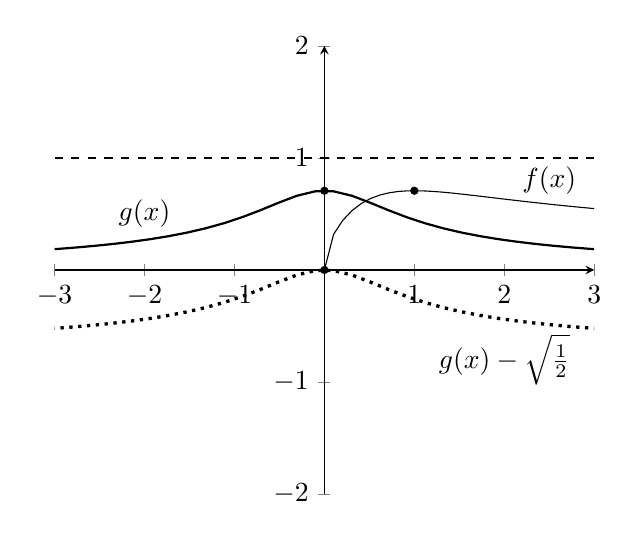
\begin{tikzpicture}[scale=1]
\begin{axis}[
    axis lines=center,
    xmin = -3,
    xmax = 3,
    ymin = -2,
    ymax = 2,
]
\addplot [
    domain=0:5, 
    samples=50, 
]
{sqrt((x)/(1+x^2))};
\addplot [
    domain=-5:5, 
    samples=50,
    thick, 
]
{(1)/(sqrt(3*x^2+2))};
\addplot [
    domain=-5:5, 
    samples=50,
    very thick, 
    dotted,
]
{(1)/(sqrt(3*x^2+2))-.707};

\draw[dashed,thick] (axis cs:-3,1) -- (axis cs:3,1);
\fill (axis cs: 0,.707) circle(1.5pt);
\fill (axis cs: 1,.707) circle(1.5pt);
\fill (axis cs: 0,0) circle(1.5pt);
\node at (axis cs: -2,.5) {$g(x)$};
\node at (axis cs: 2.5,.8) {$f(x)$};
\node at (axis cs: 2,-.8) {$g(x)-\sqrt{\frac{1}{2}}$};
\end{axis}
\end{tikzpicture}
\end{center}
ההערה "אם ידוע כי הפונקציות תחתכות בנקודה אחת בלבד" היתה לי די מוזרה, אבל לאחר מחשבה הבנתי שההערה באה למנוע אפשר של חיתוך כאשר
$x>1$
ושואף לאינסוף.

רציתי להשתכנע שאכן ההערה נכונה. כאשר משווים 
$f(x)=g(x)$
ומפשטים, מקבלים פולינום ממעלה שלישי:
\[
3x^3-x^2+2x-1=0\,.
\]
לא התחשק לי לחפש את הנוסחה )המסובכת( למציאת פתרונות למשוואות ממעלה שלישי, אבל לבסוף שמתי לב שאם
$x>1$,
$3x^3-x^2>0$
ו-%
$2x-1>0$,
ולכן לא יכול להיות פתרונות נוספים.

\textbf{סעיף ג}

הערך המינימלי של 
$f(x)$
הוא
$0$,
והערך המקסימלי של
$g(x)$
הוא
$\sqrt{\frac{1}{2}}$.
אם
$k>\sqrt{\frac{1}{2}}$
לא יהיו נקודות חיתוך בין שתי הפונקציות.


%%%%%%%%%%%%%%%%%%%%%%%%%%%%%%%%%%%%%%%%%%%%%%%%%%%%%%%%%%%%%%%%%%%%%%

\section{קיץ תשע"ד מועד ב}

\begin{center}
\selectlanguage{english}
\includegraphics[width=\textwidth]{summer-2014b-7}
\end{center}

\vspace{-2ex}

\textbf{סעיף א}

$(1)$
הפונקציה לא מוגדרת כאשר המכנה מתאפס 
$x^2-1=0$,
כאשר 
$x=\pm 1$.

$(2)$
ה%
\asms{}
האנכיות הן במקומות שהפונקציה לא מוגדרת
$x=\pm 1$.

חישוב ה%
\asm{}
האופקית:
\[
\frac{1-\frac{4}{x}+\frac{4}{x^2}}{1-\frac{1}{x^2}}\limit{\pm\infty}\frac{1}{1}=1\,.
\]

$(3)$
כאשר
$x=0$,
$y=\frac{(-2)^2}{-1}=-4$.

כאשר 
$y=0$
המכנה שונה מאפס, ולכן 
$(x-2)^2=0$
ו-%
$x=2$.

נקודות החיתוך הן
$(2,0), (0,-4)$.

$(4)$
חישוב הנגזרת הראשונה:
\[
f'(x)=\frac{2(x-2)(x^2-1)-(x-2)\cdot 2x}{(x^2-1)^2}=\frac{2(2x^2-5x+2)}{(x^2-1)^2}\,.
\]
המכנה חיובי בתחום ההגדרה ולכן נקודות הקיצון הן הפתרונות של:
\[
2x^2-5x+2=(2x-1)(x-2)=0\,.
\]
הנגזרת השנייה )של המונה( היא
$2(4x-5)$
שהיא חיובי עבור 
$x=2$
ושלילי עבור
$x=\frac{1}{2}$.
נקודות הקיצון הן:
\[
(2,0)\quad \textrm{\R{מינימום}},\quad\quad (\frac{1}{2},-3)\quad \textrm{\R{מקסימום}}\,.
\]

\np

\textbf{סעיף ב}

מה%
\asms{}
ונקודות הקיצון אפשר לצייר תרשים עבור 
$x>-1$.
עבור
$x<-1$
נבדוק אם הגרף מעל ל%
\asm{}
האופקית או מתחתיה.
$f(-2)=\frac{16}{3}>1$
ולכן הגרף מעל ל%
\asm{}.

\begin{center}
\selectlanguage{english}
\begin{tikzpicture}[scale=1]
\begin{axis}[
    axis lines=center,
    xmin = -5,
    xmax = 5,
    ymin = -5,
    ymax = 5,
]
\addplot [
    domain=-5:-1.05, 
    samples=50, 
]
{(x-2)^2)/(x^2-1)};
\addplot [
    domain=-.95:.95, 
    samples=50, 
]
{(x-2)^2)/(x^2-1)};
\addplot [
    domain=1.05:5, 
    samples=50, 
]
{(x-2)^2)/(x^2-1)};
\draw[dashed,thick] (axis cs:-1,-5) -- (axis cs:-1,5);
\draw[dashed,thick] (axis cs:1,-5) -- (axis cs:1,5);
\draw[dashed,thick] (axis cs:-5,1) -- (axis cs:5,1);
\fill (axis cs: 0,-4) circle(1.5pt);
\fill (axis cs: .5,-3) circle(1.5pt);
\fill (axis cs: 2,0) circle(1.5pt);
\end{axis}
\end{tikzpicture}
\end{center}


\textbf{סעיף ג}

אם הנגזרת הראשונה שלילית, הפונקציה יורדת, ולכן
$\frac{1}{2}< x < 1, 1<x<2$.
אם הנגזרת השנייה חיובית, הנגזרת הראשונה עולה, ולכן
$x<-1, -1<x<\frac{1}{2}, 1<x<x_1$
כאשר 
$x_1$
היא נקודת הפיתול אי-שם מימין ל-%
$x=2$.
החיתוך בין שני התחומים הוא
$1<x<2$.

\np


%%%%%%%%%%%%%%%%%%%%%%%%%%%%%%%%%%%%%%%%%%%%%%%%%%%%%%%%%%%%%%%%%%%%%%

\section{קיץ תשע"ד מועד א}

\begin{center}
\selectlanguage{english}
\includegraphics[width=\textwidth]{summer-2014a-7}
\end{center}

\vspace{-2ex}

\textbf{סעיף א}

$(1)$
הפונקציה לא מוגדר כאשר 
$ax^2+9\leq 0$.
נתון ש-%
$a>0$
אז הביטוי תמיד גדול מאפס, והפונקציה מוגדרת עבור כל 
$x$.

$(2)$
נחשב את הנגזרת הראשונה והנגזרת השנייה:
\erh{2pt}
\begin{equationarray*}{rcl}
f'(x)&=&\frac{1}{2}(ax^2+9)^{-\frac{1}{2}}\cdot 2ax= \frac{ax}{\sqrt{ax^2+9}}\\
&&\\
f''(x)&=&\frac{a\sqrt{ax^2+9}-ax\cdot \disfrac{ax}{\sqrt{ax^2+9}}}{ax^2+9}\\
&&\\
&=&\frac{a(ax^2+9)-(ax)^2}{(ax^2+9)\sqrt{ax^2+9}}=\frac{9a}{(ax^2+9)\sqrt{ax^2+9}}\,.
\end{equationarray*}
גם המונה וגם המכנה חיוביים, ולכן הנגזרת השנייה לא מתאפסת ואין נקודות פיתול.

\textbf{סעיף ב}

$(1)$
$f'(x)$
מוגדרת כאשר 
$ax^2+9>0$,
ולכן היא מוגדרת לכל 
$x$
בדיוק כמו
$f(x)$.


$(2)$
נחלק את המונה והמכנה ב-%
$\sqrt{x^2}$:
\[
f'(x)=\disfrac{\disfrac{ax}{\sqrt{x^2}}}{\sqrt{a+\disfrac{9}{x^2}}}\,.\]

\np

מכאן ש:
\[
f(x)\limit{+\infty} \frac{a}{\sqrt{a}}=+\sqrt{a},\quad\quad f(x)\limit{-\infty} \frac{-a}{\sqrt{a}}=-\sqrt{a}\,.
\]

$(3)$
ראינו בסעיף א שהנגזרת השנייה תמיד חיובית ולכן הנגזרת הראשנוה תמיד עולה.

$(4)$

\begin{center}
\selectlanguage{english}
\begin{tikzpicture}[scale=1]
\begin{axis}[
    axis lines=center,
    xmin = -4,
    xmax = 4,
    ymin = -2,
    ymax = 2,
]
\addplot [
    domain=-4:4, 
    samples=50, 
]
{x/sqrt(x^2+9)};
\draw[dashed,thick] (axis cs:-4,1) -- (axis cs:4,1);
\draw[dashed,thick] (axis cs:-4,-1) -- (axis cs:4,-1);
\end{axis}
\end{tikzpicture}
\end{center}

\textbf{סעיף ג}

האינטגרל של הנגזרת של פונקציה הוא הפונקציה עצמה.
\[
\int_{-4}^{0} 0-f'(x)dx = -\int_{-4}^{0}f'(x)dx = \left.-f(x)\right|_{-4}^{0} = -f(0) + f(-4) = 2\,.
\]
קל לחשב ש-%
$f(0)=\sqrt{9}=3$
ו-%
$f(-4)=\sqrt{16a+9}$.
הפיתוי הוא לחשב את הערך של 
$a$
אבל השאלה דורשת את הערך של
$f(-4)$
בלי לחשב את הערך של
$a$.
החישוב אפילו קל יותר
$f(-4)=2+3=5$/.
בגלל ש-%
$x$
מופיע רק כ-%
$x^2$,
$f(4)=f(-4)=5$.

מי שמעוניין יכול לחשב את ערכו של 
$a$:
\begin{eqnarray*}
\sqrt{16a+9}&=&2+3\\
a&=&1\,.
\end{eqnarray*}


\np

%%%%%%%%%%%%%%%%%%%%%%%%%%%%%%%%%%%%%%%%%%%%%%%%%%%%%%%%%%%%%%%%%%%%%%

\section{חורף תשע"ד}

\begin{center}
\selectlanguage{english}
\includegraphics[width=\textwidth]{winter-2014-8}
\end{center}

\vspace{-4ex}

\textbf{בבחינה זו היו שלוש שאלות בפרק השני לכן מספר השאלה הוא 
$8$
ולא 
$7$.}

\begin{center}
\selectlanguage{english}
\begin{tikzpicture}%[scale=.7]
\coordinate (A) at (0,0);
\draw[thick] (A) -- node[left] {$b$} (-117.5:6) coordinate (B);
\draw[thick,name path=bc] (A) -- (-62.5:6) coordinate (C);
\draw[thick] (B) -- (C);
\draw[thick] (B) -- node[above] {$d$} ($(A)!(B)!(C)$) coordinate (D);
\draw[thick] (D) -- node[left] {$e$} ($(B)!(D)!(C)$) coordinate (E);
\fill (B) node[below] {$B$} node[above right,xshift=18pt] {$x$} circle(1.5pt);
\fill (A) node[above] {$A$} node[below,yshift=-12pt] {$2x$} circle(1.5pt);
\fill (C) node[below right] {$C$} node[above right] {$90-x$} circle(1.5pt);
\draw[<-,thick] ($(C)+(-12pt,8pt)$)-- +(14pt,0);
\fill (D) node[right] {$D$} circle(1.5pt);
\fill (E) node[below] {$E$} circle(1.5pt);
\draw[thick,rotate=90] (E) rectangle +(7pt,7pt);
\draw[thick,rotate=117.5] (D) rectangle +(7pt,7pt);
\end{tikzpicture}
\end{center}

נצדיק את סימון הזוויות בתרשים. זוויות הבסיס
$\angle ACB,\angle ABC$
של המשולש שווה-שוקיים הן:
\[
\frac{180-2x}{2}=90-x\,.
\]
במשולש ישר-זווית
$\triangle BDC$,
$\angle DBC=90-(90-x)=x$.

במבט ראשון נראה שאפשר למצוא את הערך המקסימלי של
$DE=e$
על ידי מציאת הנגזרת 
$e'=(d \sin x)' = d (\sin x)'=0$.
אבל זה לא נכון כי
$d$
איננה קבוע ולכן אי אפשר להוציא אותו מהנגזרת. נתון ש-%
$b$
קבוע, כך שעלינו למצוא ביטוי מהצורה
$e=b \cdot f(x)$.

את החישוב נבצע בשני שלבים, תחילה נבטא את 
$e$
כפוקציה של
$x,d$,
ואח"כ נבטא את
$d$
כפונקציה של
$x,b$.
אפשר להשתמש בחוק הסינוסים, אבל פשוט יותר להשתמש בהגדרת הפונקציות הטריגונמטריות במשלושים ישר-זווית
$\triangle BED,\triangle BDA$:
\erh{1pt}
\begin{equationarray*}{rcl}
e&=&d\sin x\\
d&=&b\sin 2x\\
e&=&(b\sin 2x)\sin x\\
&=&b(2\sin x \cos x)\sin x=2b\sin^2 x\cos x
\end{equationarray*}
\np
\erh{1pt}
\begin{equationarray*}{rcl}
e'&=&2b(2\sin x \cos x\cos x - \sin^2 x \sin x)\\
&=&2b\sin x(2\cos^2 x-\sin^2 x)=0\,.
\end{equationarray*}

בגלל ש-%
$x$
זווית של משולש,
$0<x<180$.
הנגזרת מתאפסת אם 
$\sin x = 0$
שלא ייתכן, כי
$x=0,x=180$
אינם יכולים להיות זוויות במשולש. הנגזרת גם מתאפסת אם:
\erh{6pt}
\begin{equationarray*}{rcl}
2\cos^2 x-\sin^2 x&=&0\\
\tan x &=& \frac{\sin x}{\cos x} = \pm \sqrt{2}\\
x&=&54.74,\; 124.26\,.
\end{equationarray*}
אבל 
$\angle BAC=2x$
כך ש-%
$x=54.74$
הוא הפתרון האפשרי היחיד.

השאלה מבקשת את ערכו של הזוויות
$\angle BAC=2x=109.47$.

\np
%\end{comment}

\selectlanguage{english}

